
% LaTeX Code for Adversarial Attacks Taxonomy







\begin{figure*}[ht!]
  \centering
  \begin{minipage}[b]{0.48\textwidth}
    \centering
    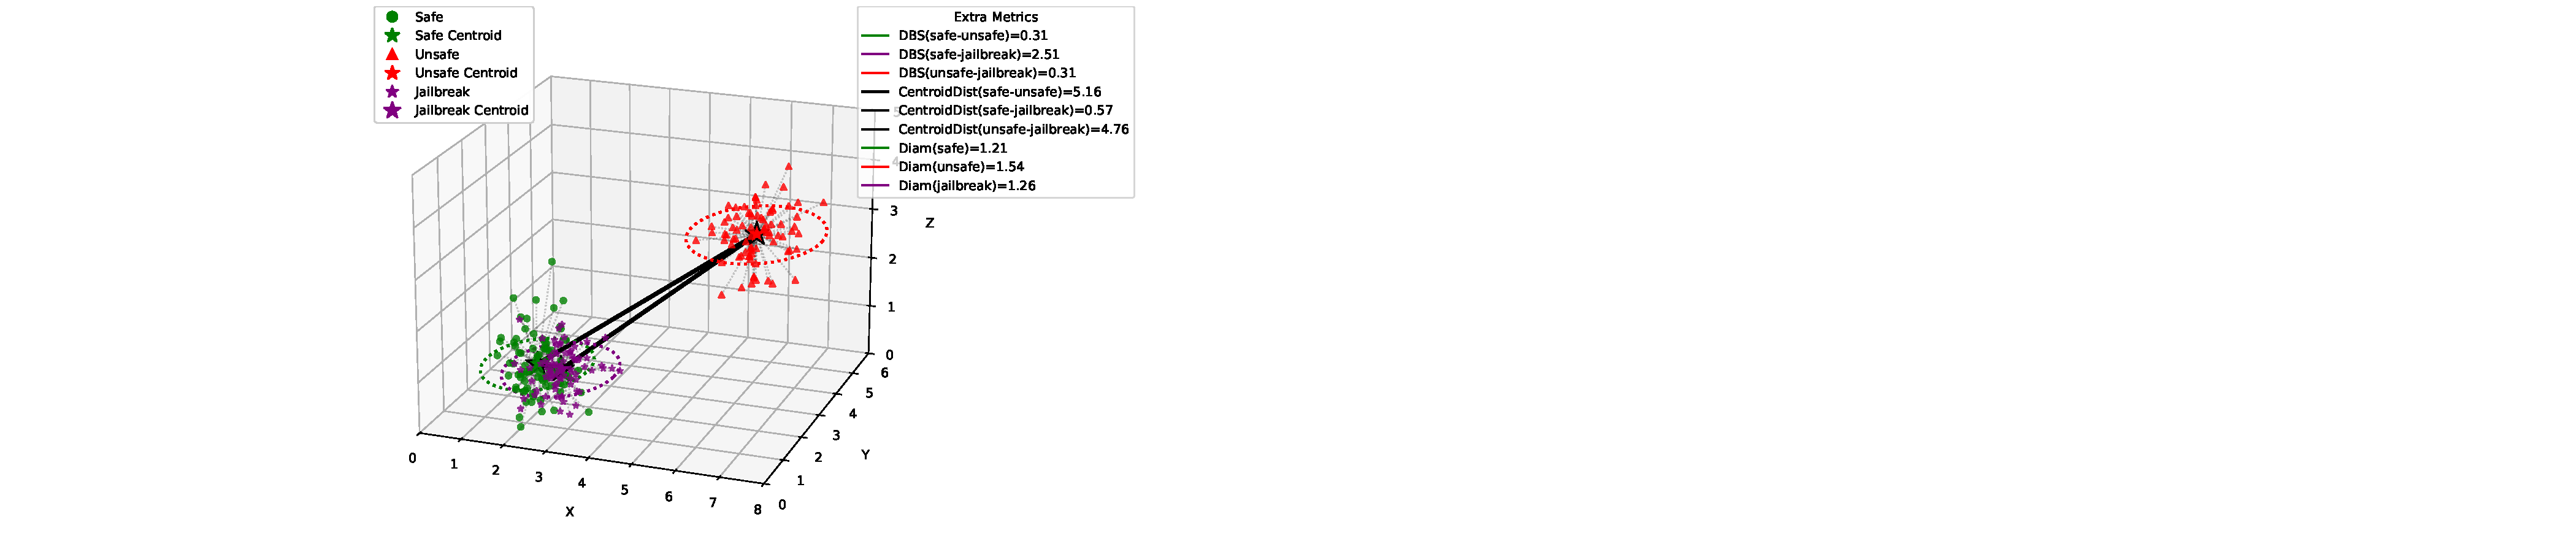
\includegraphics[width=\textwidth]{figures/left.pdf}
    \vspace{1mm}
    \centerline{\footnotesize Left: DPO Aligned LLM}
  \end{minipage}
  \hfill
  \begin{minipage}[b]{0.48\textwidth}
    \centering
    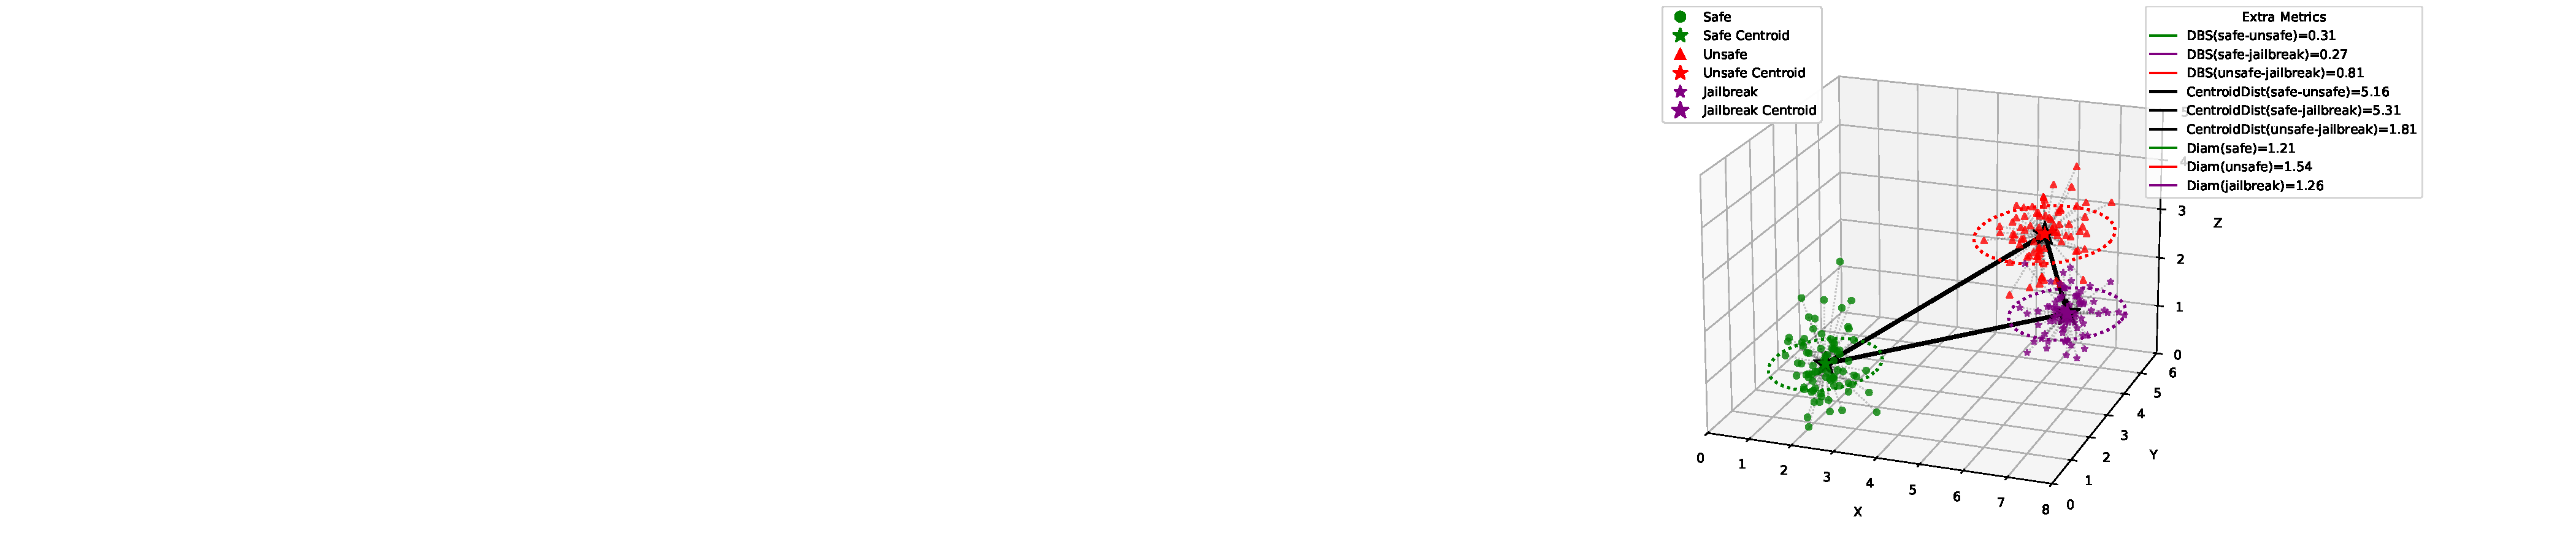
\includegraphics[width=\textwidth]{figures/right.pdf}
    \vspace{1mm}
    \centerline{\footnotesize Right: After applying GRACE (\emph{ours})}
  \end{minipage}
  \vspace{-2mm}
  \caption{
    \textbf{Comparison of Cluster Separation Before and After GRACE.}  
    \textbf{Left Panel (Vanilla DPO):} While standard DPO fine-tuning separates safe and unsafe completions (\textbf{DBS} = 0.31, \textbf{CentroidDist} = 5.16), it fails to disentangle safe from jailbreak clusters, which remain closely entangled (\textbf{DBS} = 2.51, \textbf{CentroidDist} = 0.57).  
    \textbf{Right Panel (GRACE):} GRACE reconfigures the latent space by enforcing geometric constraints, achieving clear separation between safe and jailbreak completions (\textbf{DBS} = 0.27, \textbf{CentroidDist} = 5.31), while preserving the original safe–unsafe boundary.  
    \textbf{Interpretation:} Structural metrics—DBS, centroid distances, and cluster diameters—quantitatively reveal GRACE’s capacity to align behavioral intent with latent geometry, mitigating adversarial entanglement in representational space.
}
  \label{fig:multiview_aqi_comparison}
  \vspace{-4mm}
\end{figure*}




%%%%%%%%%%%%%%%%%%%%%%%%%%%%%%%%%%%%%%%%%%%%%%%%%%%%%%%%%%%%%%%%%%%%%%%%%%




\section{Where the Firewall Cracks: A Cartography of LLM Vulnerabilities}
\label{sec:asr}

Figure~\ref{fig:grace_benchmark} reports ASRs for 21 LLMs under the {\fontfamily{uncl}\fontsize{7}{8}\selectfont ALKALI} benchmark. While frontier models like \texttt{Llama-3} and \texttt{GPT-4} show stronger resistance, instruction-tuned open models—\texttt{Vicuna}, \texttt{Mistral}, and \texttt{Phi}—consistently fail under persona hijacking, prompt chaining, and extraction-based exploits. Persistently high ASR, particularly for goal hijacking and stealth extraction, reveals structural fragility in current alignment defenses and underscores the need for latent-space hardening.

\textbf{Choices of LLMs - }  
To systematically evaluate the role of model size, architecture, and training provenance in adversarial vulnerability, we benchmarked 21 contemporary LLMs spanning diverse families and design philosophies. This includes open and proprietary models, ranging from dense transformers to mixture-of-experts architectures, covering parameter scales from 2B to 70B. The full suite comprises:  
\textbf{(i)} GPT-4o-mini~\cite{gpt-4o-mini},  
\textbf{(ii)} GPT-4,  
\textbf{(iii)} GPT-3.5~\cite{gpt4},  
\textbf{(iv–v)} Llama-3.1-70B \& 8B~\cite{llama-3.1},  
\textbf{(vi–vii)} Llama-3-70B \& 8B~\cite{llama-3},  
\textbf{(viii–x)} Llama-2-70B, 13B, \& 7B~\cite{llama-2},  
\textbf{(xi)} Vicuna-1.5~\cite{vicuna},  
\textbf{(xii)} Phi-2~\cite{phi-2},  
\textbf{(xiii)} Phi-3~\cite{phi-3},  
\textbf{(xiv)} Claude~\cite{claude},  
\textbf{(xv–xvi)} Mixtral-8$\times$7B \& 22B~\cite{mixtral},  
\textbf{(xvii–xviii)} Gemma-7B \& 2B~\cite{gemma},  
\textbf{(xix)} Mistral~\cite{mistral}, and  
\textbf{(xx–xxi)} DeepSeek \& DeepSeek-R1.


\vspace{-2mm}
\subsection{{\fontfamily{uncl}\fontsize{6}{7}\selectfont ALKALI} — Adversarial Safety Benchmark}
\label{sec:alkali}

Over the past three years, LLMs have become central to AI-driven reasoning, generation, and decision-making. As their capabilities scale, so do their vulnerabilities. A surge of recent work has revealed various adversarial threats, from jailbreaks~\citep{wei2023jailbroken, zhu2024promptbench} to indirect prompt injections~\citep{greshake2023indirect}, each revealing a distinct axis of alignment failure. Rather than curating a selective subset, we consolidate this literature into a unified, citation-grounded benchmark. {\fontfamily{uncl}\fontsize{6}{7}\selectfont ALKALI} spans 9,000 prompts across 3 macro-categories, 6 subtypes, and 15 attack families, supporting category-specific evaluation, subtype-level stress testing, and paper-level traceability for reproducibility and comparison, see Table~\ref{tab:alkali_data_breakdown} for details.




\begin{table}[ht!]
\centering
\resizebox{\columnwidth}{!}{
\begin{tabular}{@{}p{3.2cm} p{9.2cm} r@{}}
\toprule
\textbf{Category} & \textbf{Subtype \& Source(s)} & \textbf{Instances} \\
\midrule
\multirow{2}{=}{\textbf{Jailbreak}} 
  & \textit{Optimization-based}: \cite{wu2024llms, pair23, tap23} & 1,200 \\
  & \textit{Long-tail Distribution}: \cite{jiang2023promptpacker, schulhoff2023hackaprompt} & 1,500 \\
\midrule
\multirow{2}{=}{\textbf{Control Generation}} 
  & \textit{Direct Attacks}: \cite{jiang2023promptpacker, schulhoff2023hackaprompt} & 1,600 \\
  & \textit{Indirect Attacks}: \cite{chen2024pseudo, li2024pleak, greshake2023indirect} & 1,400 \\
\midrule
\multirow{2}{=}{\textbf{Performance Degradation}} 
  & \textit{Dataset Poisoning}: \cite{greshake2023indirect} & 1,800 \\
  & \textit{Prompt Injection}: \cite{greshake2023indirect} & 1,500 \\
\midrule
\textbf{Total} & — & \textbf{9,000} \\
\bottomrule
\end{tabular}
}
\caption{
\textbf{ALKALI Dataset Distribution by Adversarial Taxonomy.}  
Prompt distribution across {\fontfamily{uncl}\fontsize{7}{8}\selectfont ALKALI}'s three attack categories—\textit{Jailbreak}, \textit{Control Generation}, and \textit{Performance Degradation}, with representative subtypes linked to cited sources. Supports reproducible, category-specific evaluation of alignment vulnerabilities under structurally diverse threat models.
}
\label{tab:alkali_data_breakdown}
\vspace{-6mm}
\end{table}







